\section{TaskBox}
\label{sec:taskbox}

\begin{figure}[h!] 
	\centering
	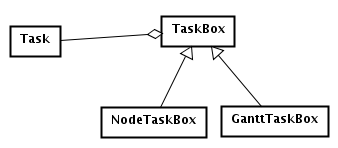
\includegraphics[width=0.5\textwidth]{../TaskBoxDetail.png}
	\caption{taskbox and its specializations}
	\label{fig:taskbox} 
\end{figure}

Il \emph{TaskBox} \`e la rappresentazione grafica di un
\emph{Task} (\autoref{fig:task}). Questo concetto astrae su queste
specializzazioni:
\begin{itemize}
\item \emph{GanttTaskBox} che ci permetter\`a di costruire la rappresentazione
in un \emph{GanttChart} conformi alle norme fissate nel documento di specifica.

\item \emph{NodeTaskBox} che ci permetter\`a di costruire la rappresentazione
in un \emph{WBSChart} e in \emph{TaskNetworkChart} alle norme fissate nel 
documento di specifica.
\end{itemize}

Abbiamo usato il principio di incapsulare il concetto che varia, modellando il
concetto astratto di \emph{TaskBox} per avere questi vantaggi:
\begin{itemize}
  \item non legare un \emph{Chart} specifico a una rappresentazione specifica
  \item aggiungere una nuova rappresentazione consiste nel modellarla e
  dichiarare che si tratta di una specializzazione di \emph{TaskBox}
  \item potremo cambiare a runtime il tipo di rappresentazione voluta nel
  disegno di un \emph{Chart}, magari inserire in un \emph{WBSChart} una
  rappresentazione pensata per i \emph{GanttChart}
\end{itemize}